\section{Background}
\label{sec:background}

%This section provides some background information on how
%\sft{ssu-align} aligns SSU sequences and how it identifies and removes
%columns from (masks) those alignments that are most likely to contain
%errors in preparation for phylogenetic analysis.  

\subsection{Profile versus nearest neighbor alignment strategies}

There are several existing software packages dedicated to
SSU alignment, including, but not limited to, \software{NAST}
\cite{DeSantis06} (used by the \software{greengenes} database
\cite{DeSantis06a}), \software{PyNast} \cite{Caporaso10},
\software{SINA} (used by the \software{silva} database
\cite{Pruesse07}), and \software{mothur} \cite{Schloss09}.
Most of these methods use a \emph{nearest-neighbor}
(NN) based alignment strategy: given a new target sequence to align,
each sequence in a reference alignment is evaluated to find one or
more nearest-neighbor template sequences that are most similar to the
target using a similarity metric such as sequence identity. An
alignment of the target sequence to its template(s) is then
computed, and this alignment is used to place the target within the
context of the full reference alignment (figure~\ref{fig:nnprof}).

In contrast, \software{ssu-align} uses a profile-based alignment
strategy: each target sequence is aligned independently to a
statistical model called a profile
(figure~\ref{fig:nnprof}). The profiles \software{ssu-align} uses for
alignment are called covariance models (CMs)
%, which model both the
%conserved sequence and secondary structure of SSU
\footnote{\textsc{ssu-align} actually uses two types of profiles,
  CMs and profile HMMs, which model only conserved primary
  sequence. Profile HMMs are used to determine which domain each
  sequence belongs to, and then the corresponding domain-specific CM
  is used to align the sequence, as depicted in
  figure~\ref{fig:schematic}.}.
A comprehensive explanation of CMs is outside the scope of this
guide. Instead, a brief discussion of some of their relevant features
for using \textsc{ssu-align} and understanding its output is included
below. For more information on CMs see
\cite{Eddy94,Durbin98,Eddy02b,NawrockiEddy07,Nawrocki09,Nawrocki09b,KolbeEddy09}.

\begin{figure}
  \begin{center}
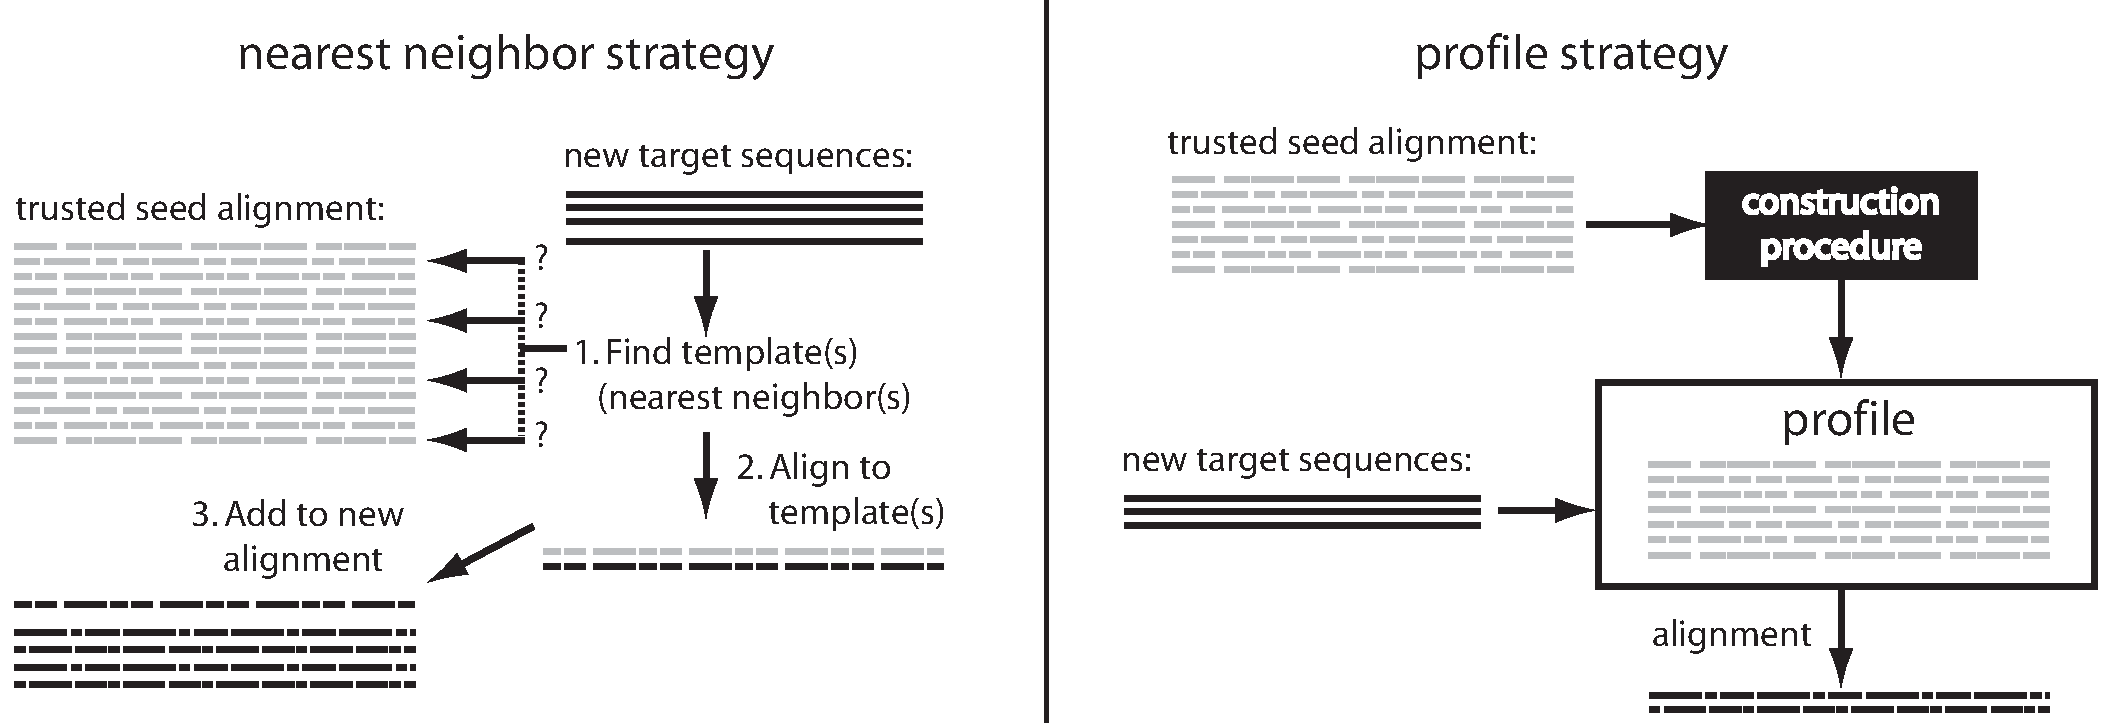
\includegraphics[width=6in]{Figures/nnprof}
  \end{center}
  \caption{Schematic of nearest-neighbor and
        profile based alignment strategies.}
  \label{fig:nnprof}
\end{figure}

\subsubsection{Covariance models: profiles of RNA sequence and secondary structure}

A CM is a consensus model of the conserved sequence and secondary
structure of an RNA family that is built from a multiple sequence
alignment. This alignment is called the \emph{seed}
alignment of the model. The seed alignment should
include a representative set of sequences from the family being
modeled and must include consensus structure annotation indicating
which positions in the alignment are basepaired to each other.  Given
a new target sequence, its best-scoring alignment to the CM can be
computed using a dynamic programming algorithm. Both primary
sequence conservation and secondary structure conservation between the target
and the model contribute to the alignment score.
%  that takes into account both the sequence and structure conservation in the
Figure~\ref{fig:toyex} depicts the building of a CM for a small,
made-up RNA family and the alignment of sequences using that CM.

The default archaeal, bacterial, and eukaryotic CMs used by
\sft{ssu-align} have 1508, 1582, and 1881 consensus positions,
respectively. Any column for which fewer than 80\% of the sequences in
the seed alignment had gaps was defined as a consensus position when
the default models were constructed\footnote{The 80\% value differs
  from the 50\% default used by the \prog{cmbuild} program of
  \sft{infernal} and the \sft{Rfam} database when building CMs.}.
The derivation of the three seed alignments and the specific method
used to build the models is discussed in detail in
section~\ref{sec:models} of this guide.

%Profiles like CMs use position-specific scores learned from the seed
%alignment for aligning each possible nucleotide in a target sequence
%to each consensus position. Basepaired positions 
%%For example, a consensus position that is
%%100\% \prog{G} in the seed alignment will assign \prog{G} a high
%%score and other nucleotides a low score, while a consensus position
%%that is 25\% \prog{A}, \prog{C}, \prog{G} and \prog{U} will assign all
%%four nucleotides marginal scores. 
%A CM also contains position-specific scores for inserting nucleotides,
%i.e. placing them in between two adjacent consensus positions, and deleting nucleotides,
%i.e. aligning a consensus position to a gap in the sequence. 
%%Whenever
%%a sequence requires an insert after a consensus column, gaps must be
%%added to accomodate that insert in the other sequences in the
%%alignment.

\subsubsection{Profiles use position-specific scores}

The scores used when aligning sequences to a CM are position-specific
and are derived from the observed nucleotide distributions in the seed
alignment. As a simple example, consider the small structural RNA
family in figure~\ref{fig:toyex}. This RNA forms the simple stem-loop
structure shown in part A of the figure. The seed alignment is in
Stockholm format. The \prog{\#=GC SS\_cons} line maps the secondary
structure onto the alignment. Basepairs in this line are indicated by
matching \prog{<} with \prog{>}, just like matching parentheses in a mathematical
formula. When a CM is built from this seed alignment, each of the
columns that include fewer than 80\% gaps will become consensus
positions of the model. There are 11 such positions in the seed
alignment, which are numbered. Other columns are considered insert columns;
these are marked with a \prog{.} in the {\#=GC SS\_cons} line, and
\prog{.} or lowercase nucleotides in the sequences. Basepaired
positions in the structure will become consensus basepairs, and other
positions will be single-stranded consensus positions. 

Each single-stranded consensus position of the model will include
scores for aligning to each of the four possible nucleotides:
\prog{A}, \prog{C}, \prog{G}, and \prog{U}, based on their frequency
in the corresponding position of the alignment. For example, column 5
includes an \prog{A} in all 8 sequences in the seed alignment and so
would assign high scores to \prog{A} and low scores to the other three
nucleotides. In contrast, column 7, which includes two cases of each
of the four nucleotides would assign equal, marginal scores to all
four nucleotides.  Importantly, basepaired positions will assign
scores to two nucleotides at once and so will include scores for each
of the 16 possible pairs of nucleotides. For example, the pair between
positions 1 and 11 is 100\% \prog{GC} in the seed alignment and so
\prog{GC} pairs in the target would receive high scores, while the
other 15 possible pairs would receive low scores. In contrast, the
pair between positions 3 and 8 includes two of each of the four
possible Watson-Crick basepairs: \prog{AU}, \prog{UA}, \prog{CG}, and
\prog{GC}, and so these four basepairs would receive high scores,
while the other 12 possible pairs would receive lower
scores. Additionally, position-specific scores for inserting
nucleotides are derived from the alignment. Positions 5 and 9 are the
only two after which any insertions occur in the alignment, and so the
score for inserts after those positions would be be higher than for
the other positions. Similarly, the only deletions, i.e. gaps in
consensus positions, occur at positions 4 and 6, with one occuring in
6, and three in 4. Consequently, the deletion score for position 6
would be highest, with deletes in 4 receiving lower scores, and all
other positions receiving still lower scores. This discussion is
oversimplified for brevity. For formulas and more details on how 
the position-specific scores are calculated, see \cite{Durbin98,Nawrocki09}.

In contrast, nearest-neighbor based methods often do not use
position-specific scores. For example, if a single template sequence
is used,  aligning an \prog{A} in the target to any \prog{A} in the
template sequence will be given the same score. This is because, given
one template sequence, there is no way for the method to distinguish
the relative level of conservation at different positions.

Pairwise alignment with position-independent scores is accurate when
the template is nearly identical to the target, but becomes more
difficult as that identity decreases. As a result, most
nearest-neighbor based methods use very large reference alignments
(thousands of sequences) to increase the probability that a nearly
identical template exists for any potential target. Ensuring the
accuracy of such large reference alignments is critical 
but time-consuming and requires expert curators. 
Seed alignments for profile-based methods on the other
traditionally include less than one hundred sequences
\cite{Finn10,Gardner09}.
%In fact, the
%\sft{pfam} and \sft{rfam} databases collectively include over 12,000
%separate seed alignments, the vast majority of which contain fewer
%than 100 sequences. 

\subsection{Two types of alignment columns: consensus and inserts}

Alignments created by \sft{ssu-align} will contain two types of
columns: consensus columns, that correspond to a consensus position of
the model, and insert columns, which include nucleotides inserted
between consensus positions of the model. These columns can be
distinguished based on the \prog{\#=GC RF} line in the alignment
files. Continuing with the small RNA example, figure~\ref{fig:toyex}
shows an alignment of 4 target sequences (part B) and 6 target
sequences (part C) to the CM. Notice that for both alignments, the
\prog{\#=GC RF} line contains 11 nucleotides, one for each of the
consensus columns in the model. These are the highest scoring
nucleotides at each position. Uppercase letters in this line were
highly conserved in the seed alignment, lowercase letters were less
well conserved. Positions that are gaps in the {\#=GC RF} line
contain inserted nucleotides that don't align to any of the consensus
positions. 
\sft{SSU-ALIGN} alignments created with the same CM will
always include the same number of consensus columns, but the number of
insert columns will vary depending on the input sequences.

There are two important caveats regarding how CMs and \sft{SSU-ALIGN}
treat inserts:

\begin{enumerate}
\item 
Nucleotides in insert columns are simply inserted, not aligned.

You might have noticed that the nucleotides in the insert columns x
and x are obviously misaligned with respect to each other. This is
because \sft{ssu-align} does not align inserts. Instead, inserted
nucleotides are split in half, the left half is placed flush-left next
to nearest consensus column on the left (\prog{xx} in sequence x), and
the right half is placed flush-right next to the nearest consensus
column to the right (\prog{x} in sequence y). This is an important
limitation of profile-based alignment. A nearest-neighbor based
method might be able to correctly align nucleotides that would be
inserts for a profile. However, inserted positions
should be rare. Remember that consensus positions were defined as any
position that had a nucleotide in at least 20\% of the seed
sequences, so if the seed was representative the most common inserts
should only appear in about 20\% of sequences. And if the alignment will
eventually be used for phylogenetic inference, inserted columns should
be removed first anyway, and so are unimportant. This is discussed
further below in the section on masking alignments.

\item 
Deeper alignments tend to have more insert columns. 

Because the likelihood of a large insertion in at least one sequence
increases as more sequences are added, alignments of large numbers of
sequences (deep alignments) tend to have a lot of insert columns. In
fact, the number of insert columns can routinely be greater than the
number of consensus columns. This contrasts markedly with the popular
nearest-neighbor based aligners \sft{nast} and \sft{sina}, which
generate alignments of a fixed with (7,682 columns for \sft{nast} and
50,000 for \sft{sina}). However to guarantee a fixed width, \sft{nast}
must deliberately introduce errors in the alignment in some cases
\cite{DeSantis06}. 

\end{enumerate}

\begin{figure}
\begin{center}
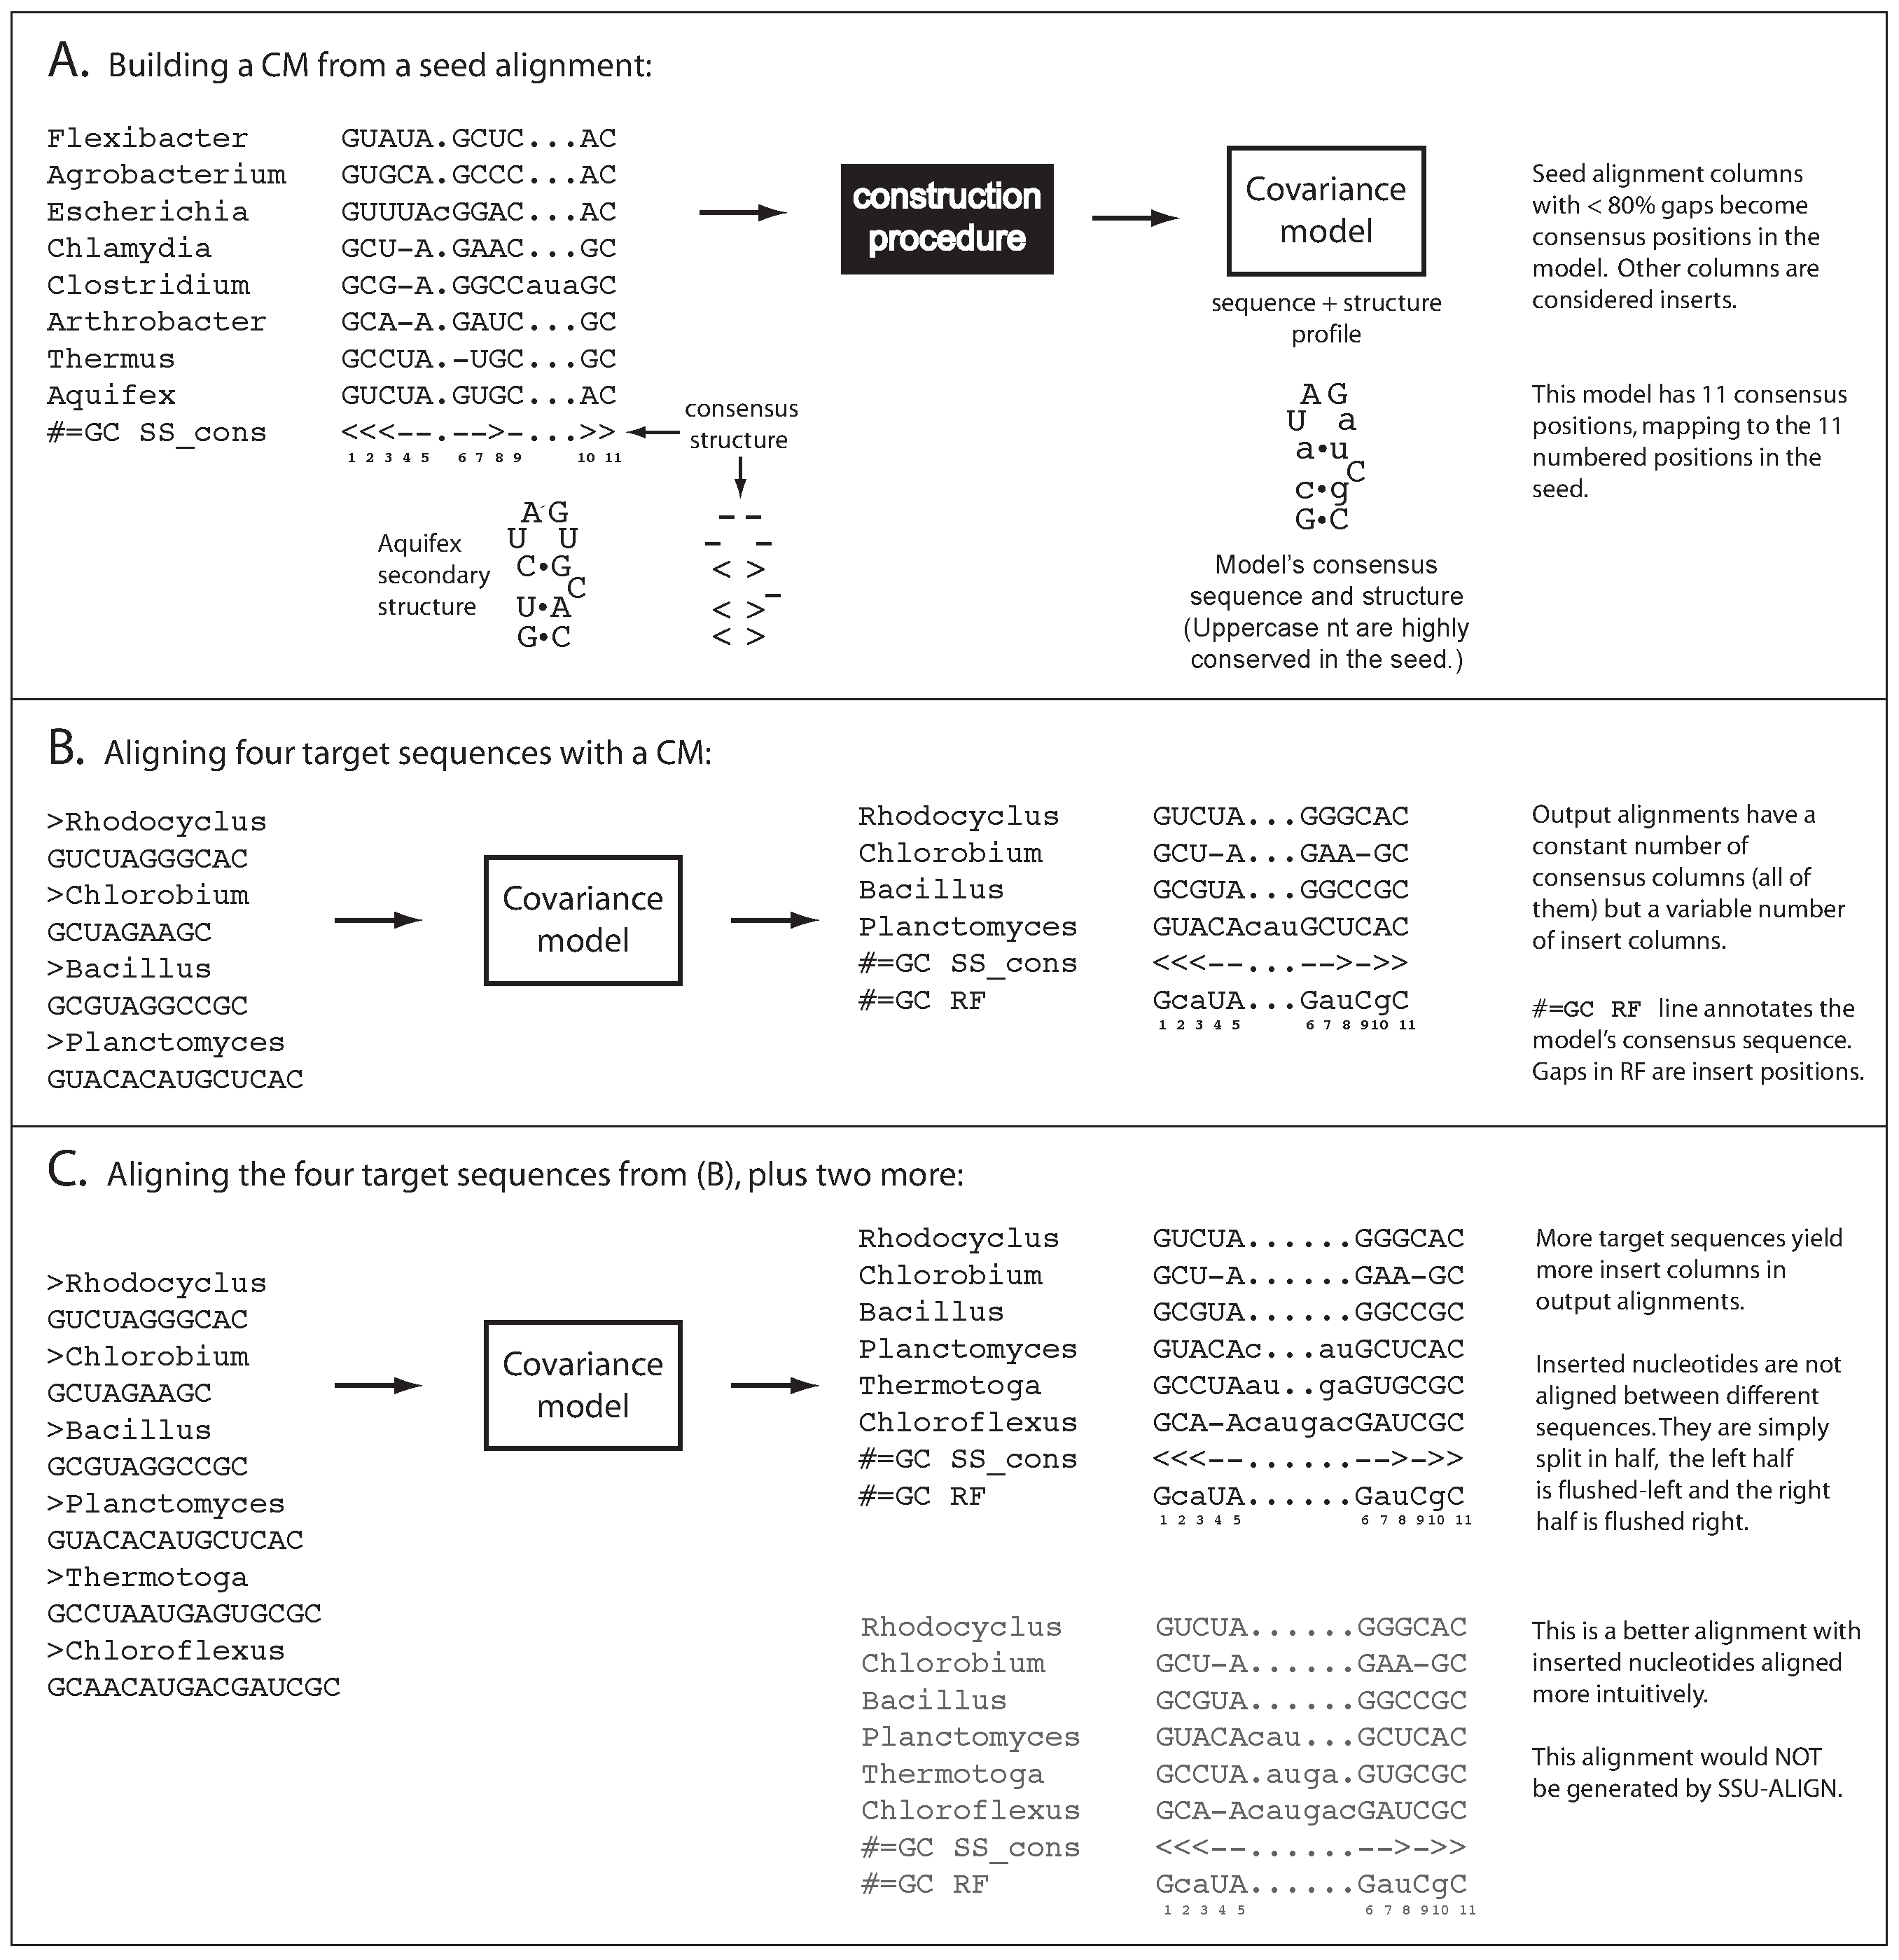
\includegraphics[height=7in]{Figures/sa-toy-example}
\caption{Building and aligning sequences to an example CM.}
\end{center}
\label{fig:toyex}
\end{figure}


\subsection{Alignment posterior probabilities are confidence estimates}
\label{sec:background-pp}

Because CMs are probabilistic models, when aligning a sequence to a CM
the posterior probability that each nucleotide aligns to each position
of the model can be calculated. 
These are \emph{confidence estimates} that each
nucleotide is correctly aligned, given the parameters of the CM. The
estimates are useful for identifying and removing columns of the
alignment that are most likely to contain errors, a procedure called
alignment \emph{masking}. Masking is especially important prior to
using the alignment as input to a phylogenetic inference program
because those programs typically assume that all nucleotides in a
given alignment column are homologous and are thus confounded by 
alignment errors. \prog{ssu-align} output alignments include posterior
probabilities that can be used to automatically construct and apply
masks using the \prog{ssu-mask} program. The tutorial
(section~\ref{sec:tutorial} includes an example of alignment masking. 


\subsubsection{Inserted columns should always be excluded during masking}

Importantly, any CM alignment mask should automatically exclude 
every insert column of the alignment. This is because, as discussed
earlier, CMs do not actually align inserted nucleotides between
different sequences, but rather simply insert them between the
appropriate consensus columns in the alignment
(figure~\ref{fig:toyex}. This means that sequence nucleotides
appearing in the same insert alignment columns are not aligned with
respect to each other and consequently should be removed prior to
phylogenetic analysis which assumes aligned nucleotides are
homologous. 

\subsubsection{Consensus columns with low alignment confidence should
  also be removed during masking}

It is necessary but not sufficient to only remove all insert columns
during masking. Additionally, some consensus columns may include
a significant number of nucleotides aligned with low confidence
estimates and these should be removed as well. 
Low alignment confidence tends to occur at positions with low sequence
conservation where insertions and deletions are common, 
corresponding to regions of the molecule that exhibit high length
heterogeneity across different species. 
In such cases, the correct alignment is often ambiguous.
Take for example the CM alignment
of the {\tt GUAU} subsequence of the \emph{Desulfovibrio
desulfuricans} SSU target sequence to a loop region depicted in
Figure~\ref{fig:ambiguity}. The reference (consensus) sequence for the
loop ({\tt AUUCAAC}) differs from {\tt GUAU} in both sequence and
length. Consequently, the CM alignment for this loop is not well
defined, and two alternative alignments are given posterior
probabilities of $0.4$ or higher.  In contrast, the surrounding helix
region, for which higher sequence similarity exists between the
reference and target sequence, is aligned confidently with high
posterior probabilities.

%Additional examples of the correlation between length heterogeneity
%and low alignment confidence are shown in figures~\ref{fig:mask-arc},
%\ref{fig:mask-bac} and \ref{fig:mask-euk}. These masks were derived as
%described in section~\ref{sec:masks}.

\begin{figure}
\ttfamily
\footnotesize
\begin{center}
%ORIGINAL DATA is from Macbook: 
%/Users/nawrockie/school/notebook/9_0309_ths/latex/ssu/ambiguity_example
\begin{tabular}{ll}
00904::Desulfovibrio\_desulfuricans-1 &                         GAUGUCGGGGA--GUAU---UCUUCGGUGUC \\
\#=GR 00904::Desulfovibrio\_desulfuricans-1 PP &                ***********--6666---9********** \\
& \\
00904::Desulfovibrio\_desulfuricans-2          &                GAUGUCGGGGA---GUAU--UCUUCGGUGUC \\
\#=GR 00904::Desulfovibrio\_desulfuricans-2 PP &                ***********---4444--9********** \\
& \\
\#=GC SS\_cons                        &                             <<<<<<<<<<<<.......>>>>>>>>>>>> \\
\#=GC RF                              &                             GGUGUuGGgggcAuUcaACgcccUCaGUGCC \\
\end{tabular}
\rmfamily

\vspace{0.2in}
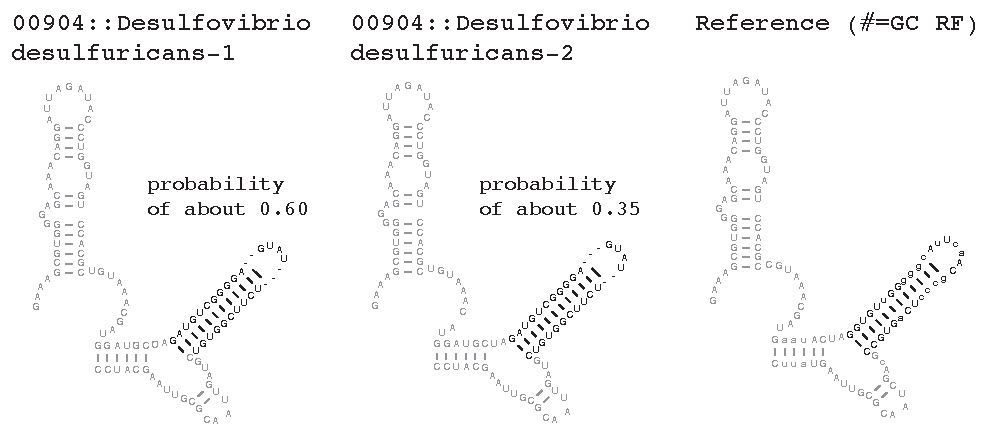
\includegraphics[width=5.7in]{Figures/ambiguity}

\caption[Example of alignment ambiguity in a hairpin loop.]{
  \textbf{Example of alignment ambiguity in a hairpin loop.}  Top: An
  alignment fragment of two different alignments of the
  \emph{Desulfovibrio desulfuricans} (sequence accession
  \texttt{M34113}) sequence from the \sft{ssu-align} bacterial seed
  alignment for the region between consensus columns $861$ and $881$.
  Each alignment is annotated with its posterior probability in the
  \texttt{\#=GR PP} rows.  Characters in PP rows have 12 possible
  values: "0-9", "*", or ".". If ".", the position corresponds to a
  gap in the sequence. A value of "0" indicates a posterior
  probability of between 0.0 and 0.05, "1" indicates between 0.05 and
  0.15, "2" indicates between 0.15 and 0.25 and so on up to "9" which
  indicates between 0.85 and 0.95. A value of "*" indicates a
  posterior probability of between 0.95 and 1.0. Higher posterior
  probabilities correspond to greater confidence that the aligned
  nucleotide belongs where it appears in the alignment.  For example,
  the second \texttt{A} in the first aligned sequence has a PP value
  of '6' indicating a posterior probability of between 0.55 and 0.65
  of being aligned in its current position. The
  probability this \texttt{A} aligns in the next position over, as it
  does in the second alignment, is between 0.35 and 0.45 as indicated
  by the 4 in that position.  The \texttt{\#=GC
  SS\_cons} and \texttt{\#=GC RF} rows correspond to the consensus
  secondary structure and sequence respectively.  
%The alignments were
%  created using \texttt{cmalign} to align this sequence to the
%  bacterial CM with the \texttt{--sample} option.  
  Bottom: The
  secondary structures corresponding to the two possible alignments of
  the \emph{D. desulfuricans} and the reference alignment.  Nucleotides
  in the actual alignment are black. Nucleotides surrounding the
  alignment fragment are gray.}
\end{center}
\label{fig:ambiguity}
\end{figure}

\subsubsection{Automated probabilistic masking with \prog{ssu-mask}}

The default masking strategy used by \prog{ssu-mask} is to remove all
insert columns and any consensus column \emph{x} for which fewer than 95\% of
the sequences that are nongaps in \emph{x} have a posterior
probability of less than 0.95 (i.e. any value in the \prog{PP}
annotation that is not \prog{*}). Columns that are 100\% gaps are also
removed. These thresholds were chosen based on good performance using
a simple SSU benchmark. See chapter 9 of \cite{Nawrocki09} for
benchmark details. The thresholds can be changed with the \prog{--pf} and
\prog{--pt} options to \prog{ssu-mask}. Additionally, columns that include
greater than a given fraction of gaps can also be removed using the
\prog{--gapthresh} option. See the \prog{ssu-mask} manual page at the
end of this guide for more details.

Alternatively, it can be useful to apply a preset mask that is not
alignment-specific so that alignments of different datasets can be
directly compared. \sft{ssu-align} includes a default preset mask for
each of the default archaeal, bacterial, and eukaryotic
alignments. The determination of these is discussed in
section~\ref{sec:masks}. 

\subsection{Other useful references}

For more information on CM parameterization and alignment, see the
\software{infernal} user's guide \cite{infernalguide}.  My
Ph.D. thesis
(\htmladdnormallink{http://selab.janelia.org/publications.html}{http://selab.janelia.org/publications.html})
includes more background on SSU databases, alignment methods, CM
acceleration heuristics used by \sft{ssu-align}, and the masking
benchmark mentioned earlier.  Other useful references on CMs include
\cite{Eddy94,Eddy02b,NawrockiEddy07,Nawrocki09,KolbeEddy09}. Finally,
publications related to the \sft{rfam} database
(\htmladdnormallink{http://rfam.sanger.ac.uk/}{http://rfam.sanger.ac.uk/}),
which uses \software{infernal} to search for and align structural RNAs
using more than 1000 different CMs, may be of interest
\cite{Griffiths-Jones03,Griffiths-Jones05,Gardner09}.


